\documentclass[
	11pt,				% tamanho da fonte
	openright,			% capítulos começam em pág ímpar (insere página vazia caso preciso)
	oneside,			% twoside para impressão em verso e anverso. Oposto a oneside
	a4paper,			% tamanho do papel. 
	% -- opções da classe abntex2 --
	%chapter=TITLE,		% títulos de capítulos convertidos em letras maiúsculas
	%section=TITLE,		% títulos de seções convertidos em letras maiúsculas
	%subsection=TITLE,	% títulos de subseções convertidos em letras maiúsculas
	%subsubsection=TITLE,% títulos de subsubseções convertidos em letras maiúsculas
	% -- opções do pacote babel --
	english,			% idioma adicional para hifenização
	french,				% idioma adicional para hifenização
	spanish,			% idioma adicional para hifenização
	brazil,				% o último idioma é o principal do documento
	]{abntex2}

\usepackage{abntex2-cefetmg-timoteo}

\usepackage{subcaption}

\usepackage{relsize}%Felipe colocou
\usepackage{float}%Felipe colocou
%\usepackage{enumitem}%Felipe colocou
%\usepackage[shortlabels]{enumitem}%Felipe

\usepackage{amsmath}
\usepackage{cmap}				% Mapear caracteres especiais no PDF
\usepackage{lmodern}			% Usa a fonte Latin Modern			
\usepackage[T1]{fontenc}		% Selecao de codigos de fonte.
\usepackage[utf8]{inputenc}		% Codificacao do documento (conversão automática dos acentos)
\usepackage{lastpage}			% Usado pela Ficha catalográfica
\usepackage{indentfirst}		% Indenta o primeiro parágrafo de cada seção.
\usepackage{color}				% Controle das cores
\usepackage{graphicx}			% Inclusão de gráficos
\PassOptionsToPackage{normalem}{ulem} % Para não usar sublinhado em referências bibliográficas
\usepackage{ulem}
\usepackage{multicol}
\usepackage{helvet}
\usepackage{multirow}
\renewcommand{\familydefault}{\sfdefault}

% Centralizando legenda das figuras (10/04/2020)
\usepackage[position=top]{subfig}

\usepackage[brazilian,hyperpageref]{backref}	 % Paginas com as citações na bibl
\usepackage[alf,abnt-thesis-year=both,]{abntex2cite}	% Citações padrão ABNT

\usepackage{longtable}

% ---
% Configurações do pacote backref
% Usado sem a opção hyperpageref de backref
\renewcommand{\backrefpagesname}{Citado na(s) página(s):~}
% Texto padrão antes do número das páginas
\renewcommand{\backref}{}
% Define os textos da citação
\renewcommand*{\backrefalt}[4]{
	\ifcase #1 %
		Nenhuma citação no texto.%
	\or
		Citado na página #2.%
	\else
		%Citado #1 vezes nas páginas #2.%
		Citado nas páginas #2.%
	\fi}%

% Inserção de imagens
% #1 -> Escala da figura
% #2 -> Nome da figura (Dentro do diretório de figuras)
% #3 -> Legenda da figura
% #4 -> Nome de referência da figura
% #5 -> Fonte da figura
% Exemplo de uso: \image{1.4}{neuronio-biologico.png}{Ilustração do neurônio biológico}{figure:bioneuron}{\citeonline{Remes2016}}
\newcommand{\image}[5]{
    \begin{figure}[H]%[h]
        \begin{center}
        \caption{#3}
        \includegraphics[scale=#1]{#2}
        \label{#4}
        \fonte{#5}
        \end{center}
    \end{figure}
}
% ---

% ---
% Informações de dados para CAPA e FOLHA DE ROSTO
% ---
\titulo{Modelando epidemias usando autômatos celulares}
\uppercase{\autor{\textbf{Arturo Sanchez \\ Felipe Menino Carlos}}}
\local{São José dos Campos}
\data{2020}

% --- 

% --- 
% Espaçamentos entre linhas e parágrafos 
% --- 

% O tamanho do parágrafo é dado por:
\setlength{\parindent}{1.3cm}

% Controle do espaçamento entre um parágrafo e outro:
\setlength{\parskip}{0.2cm}  % tente também \onelineskip

% ---
% compila o indice
% ---
\makeindex 
% ---

% ----
% Início do documento
% ----
\begin{document}

% Retira espaço extra obsoleto entre as frases.
\frenchspacing 

% ----------------------------------------------------------
% ELEMENTOS PRÉ-TEXTUAIS
% ----------------------------------------------------------
 \pretextual

% ---
% Capa
% ---
\imprimircapa

%%% no extra space before the entry, or in the LoF/LoT
% \setlength{\cftbeforechapterskip}{0pt plus 0pt} %afeta sumário, o que não desejo!
 \renewcommand*{\insertchapterspace}{} %afeta apenas lista de figuras e lista de tabelas, precisamente o que desejo!

% \pdfbookmark[0]{\listfigurename}{lof}
% \listoffigures*
% \cleardoublepage
% ---

% ---
% inserir lista de tabelas
% ---
% \pdfbookmark[0]{\listtablename}{lot}
% \listoftables*
% \cleardoublepage
% ---

% ---
% inserir lista de abreviaturas e siglas
% ---
% \begin{siglas}
%  \item[Fig.] Area of the $i^{th}$ component
%  \item[456] Isto é um número
%  \item[123] Isto é outro número
%  \item[lauro cesar] este é o meu nome
% \end{siglas}
% ---

% ---
% inserir lista de símbolos
% ---
%\begin{simbolos}
%  \item[$ \Gamma $] Letra grega Gama
%  \item[$ \Lambda $] Lambda
%  \item[$ \zeta $] Letra grega minúscula zeta
%  \item[$ \in $] Pertence
%\end{simbolos}
% ---

% ---
% inserir o sumario - Comentei essas linhas
% para add sumário só descomentar
% ---
%\pdfbookmark[0]{\contentsname}{toc}
%\tableofcontents*
%\cleardoublepage
% ---



% ----------------------------------------------------------
% ELEMENTOS TEXTUAIS
% ----------------------------------------------------------
\textual

% ----------------------------------------------------------
% Introdução
% ----------------------------------------------------------


\chapter{Introdução}

% Diferentes contextos de utilização dos autômatos celulares;
% Falar especificamente da utilização de CA para a simulação de epidemias;
% Objetivo: O presente trabalho tem como objetivo realizar a implementação e análise do modelo de CA apresentado em White et al (2007). Duas implementações do modelo foram feitas, uma utilizando Python e outra a plataforma de modelagem TerraME.

\chapter{Autômatos celulares}

\par Autômatos celulares são modelos matemáticos que tornam possível a representam de sistemas e fenômenos dinâmicos \cite{Melotti2009, Castro2008}, tornando esses ferramentas úteis para a modelagem de diferentes tipos de comportamento, sendo empregados nos mais variados contextos \cite{Castro2008}. Por sua capacidade de expressar comportamentos dinâmicos, os ACs são frequentemente descritos como contrapartes às equações diferenciais \cite{Melotti2009}, sendo utilizados em muitos trabalhos por conta de sua fácil representação e grande poder de expressão de diferentes comportamentos. \citeonline{Melotti2009} afirma que, a ideia por trás da utilização de ACs para a descrição de sistemas e fenômenos é buscar fazer a representação desses não por meio de equações complexas, mas sim, simular tais sistemas e permitir que a interação do mesmo entre seus componentes, por meio de regras simples, gere os mesmos comportamentos que estão sendo modelados.
\par Esta seção apresenta os principais fundamento para a utilização de autômatos celulares.

\section{Componentes de um autômato celular}

\citeonline{Liu2008} especifica que os autômatos celulares possuem cinco elementos fundamentais em sua composição, sendo eles: (i) Célula; (ii) Estado; (iii) Vizinhança; (iv) Regra de transição; e (v) Tempo.

\par As \texttt{Células} representam um elemento básico de um autômato celular \cite{Leite2016}. Tal componente pode ser representado em conjuntos, espacialmente dispostos em \textit{grids} \textit{n}-dimensional \cite{Shiffman2012} chamados de espaço celular \cite{Liu2008}, podendo ser composto por diferentes tipos geométricos \cite{Melotti2009}. Cada componente do espaço celular está vinculada a um \texttt{Estado}, que representa os atributos que o sistema pode assumir.
\par A \texttt{Vizinhança} determina a interação entre as células dentro de um espaço celular. Considerando os espaços celulares bidimensionais, utilizados no contexto deste trabalho, existem duas principais formas de vizinhança \cite{Leite2016}, Von Neumann e Moore, que criam as relações em um dado espaço dimensional conforme apresentado na Figura \ref{figure:neighbor}.

\begin{figure}[H]
    \centering
    \caption{Vizinhanças bidimensionais}
    \subfloat[Moore]{{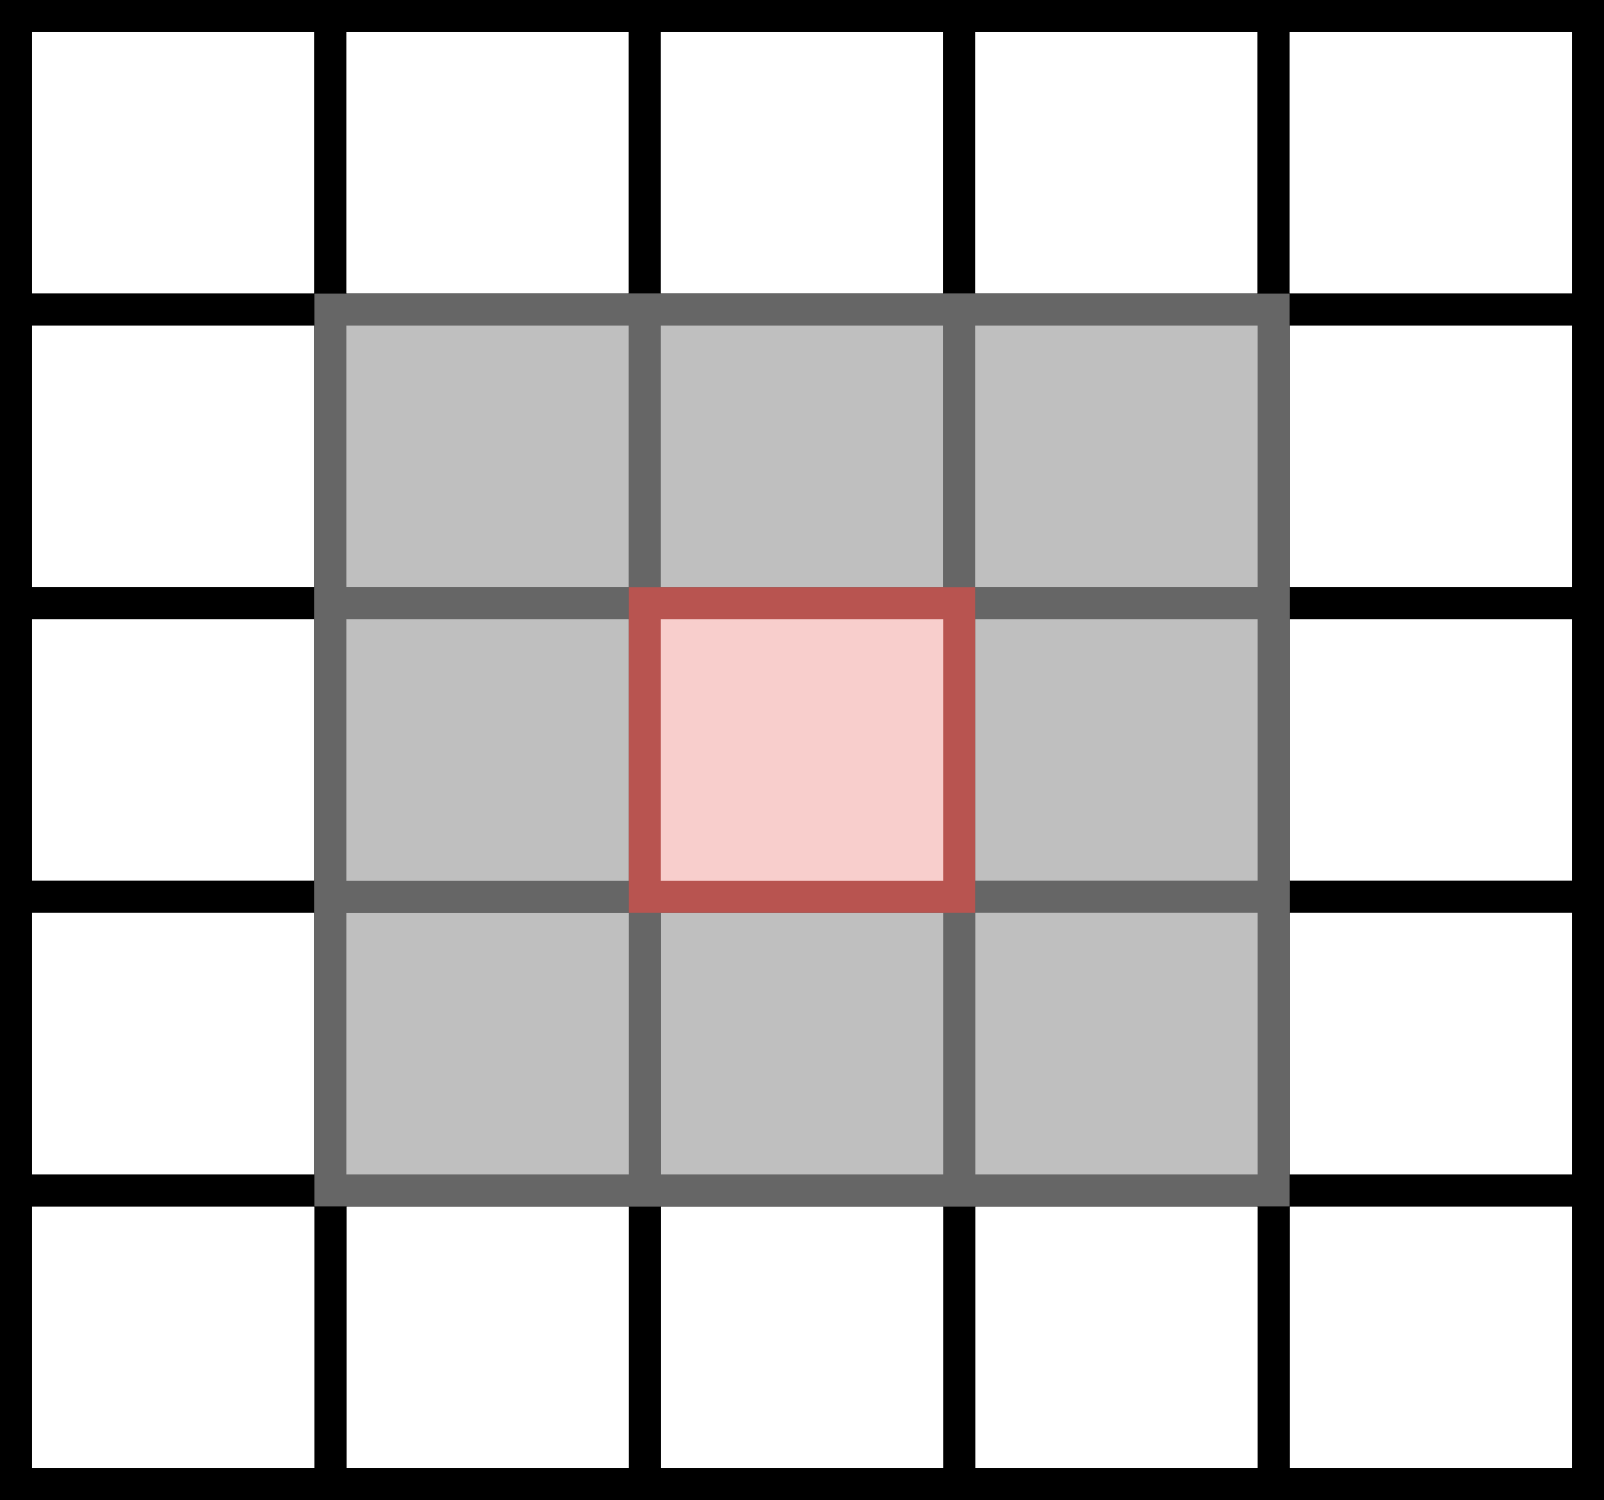
\includegraphics[height=5cm, width=5cm]{images/moore.png}}}
    \qquad
    \subfloat[Von Neumann]{{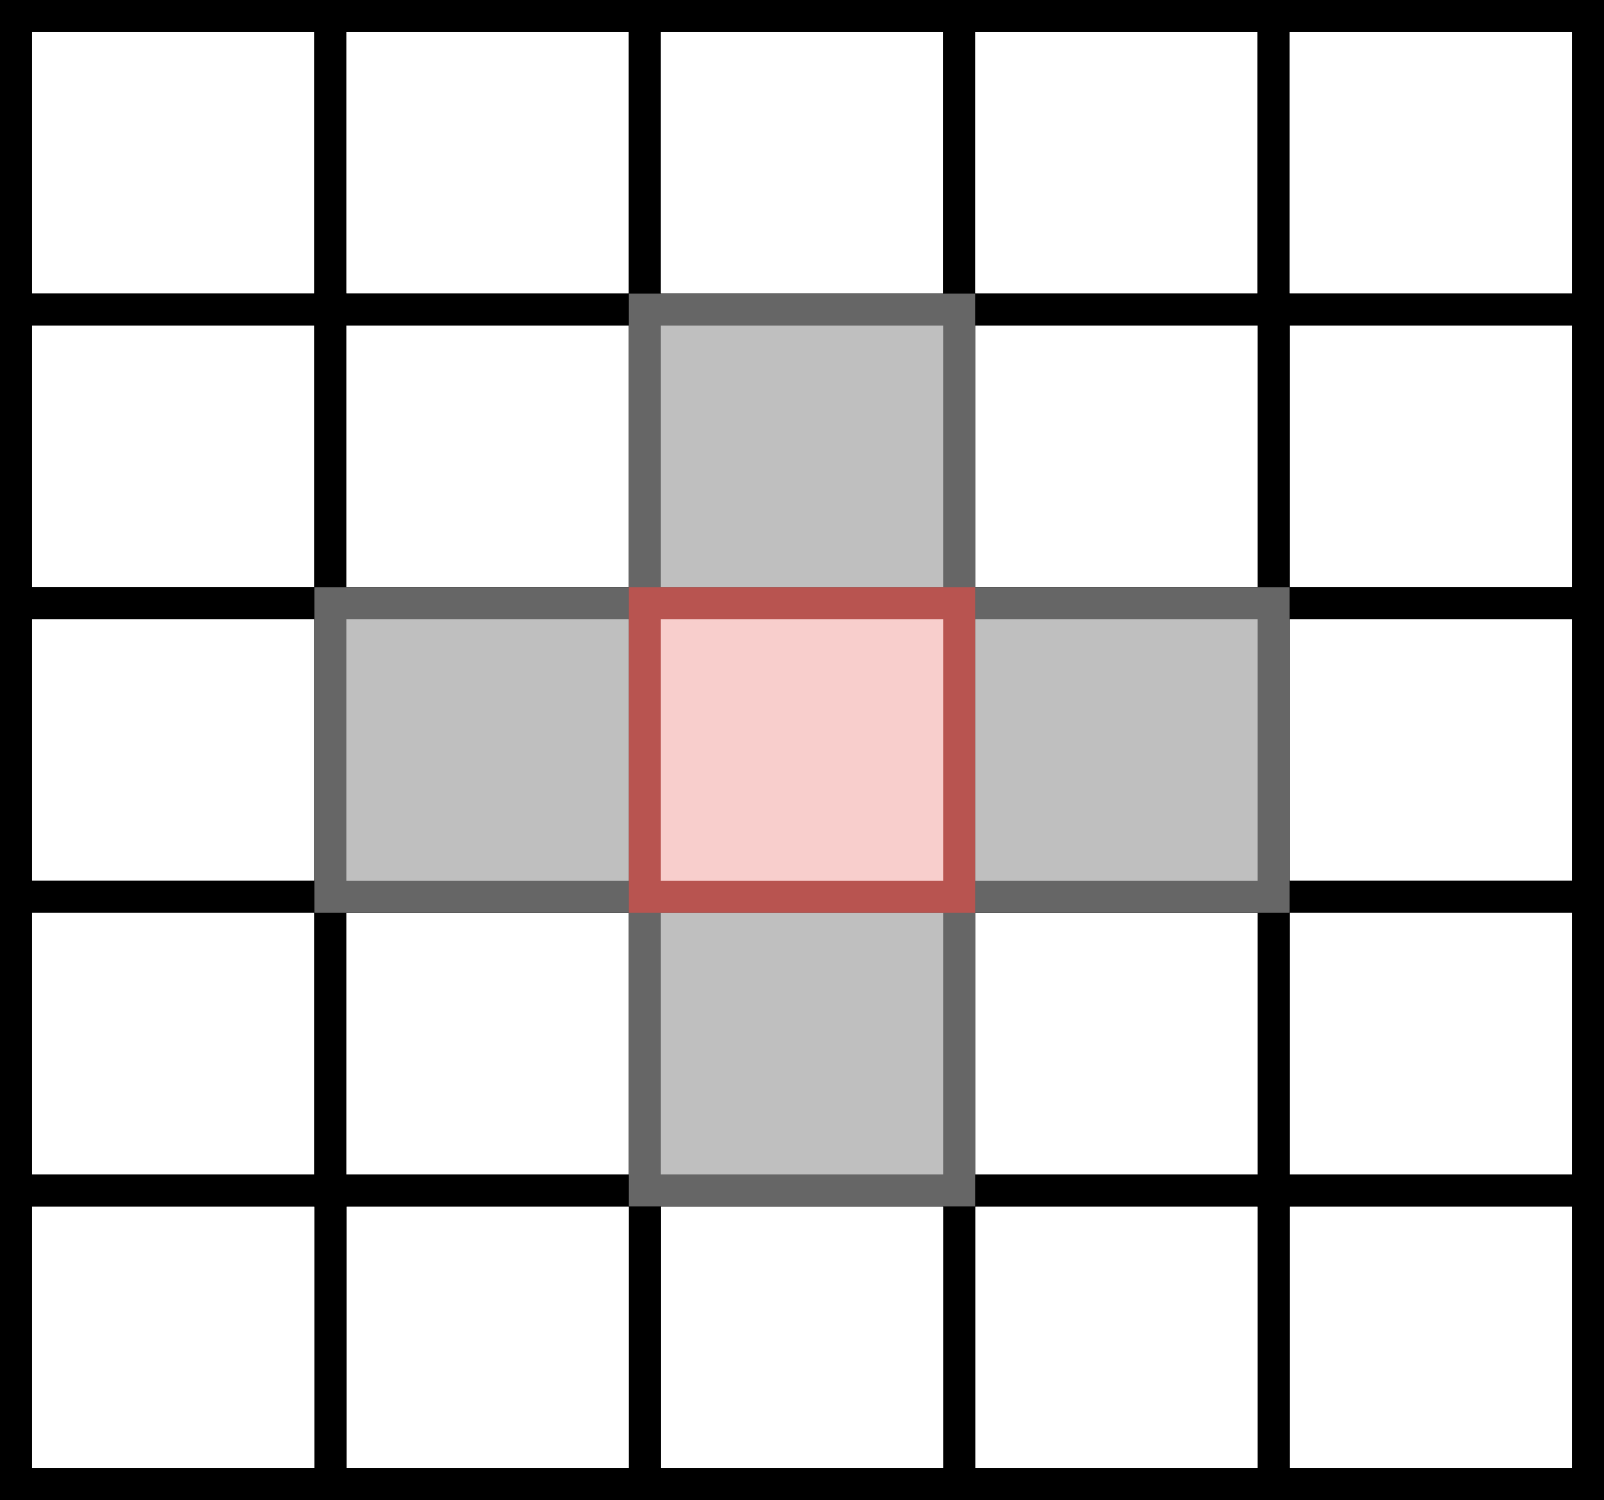
\includegraphics[height=5cm, width=5cm]{images/vonneumann.png} }}
    \qquad
    \label{figure:neighbor}
    \fonte{Adaptado de \citeonline{alexanderschatten2008}}
\end{figure}

\par Através do espaço celular e do conceito de vizinhança as \texttt{Regras de transição} podem ser definidas, essas que através de um conjunto de condições, que considerando o estado atual de cada célula e a de seus vizinhos, faz atualizações de estado em cada célula, sendo que, o estado atual sempre é definido pela análise dos estados anteriores \cite{Shiffman2012}.

\par O último componente é o \texttt{Tempo}, considerado como uma dimensão do autômato celular, é utilizado para determinar, em mudanças discretas \cite{alexanderschatten2008}, a atualização dos estados através da aplicação das regras de transição, essas sendo feitas todas ao mesmo tempo, para todas as células \cite{Liu2008}, de modo que, a atualização de um estado em um determinado tempo, não interfira. no resultado de outro no mesmo instante de tempo.

\chapter{Modelos de autômatos celulares para propagação epidêmica}

\par De acordo com \citeonline{White2007} e \citeonline{Sirakoulis2000}, modelos clássicos de propagação epidêmica podem não representam o problema como um todo, isso porque, ao aplicar equações diferenciais (Ordinárias ou Parciais), algumas características de epidemias são deixados de lado, a citar: (i) O processo de contato individual; (ii) comportamentos individuais; (iii) aspectos espaciais da propagação; e (iv) efeito dos padrões de mistura dos indivíduos.

\par Para contornar tais problemas, é proposto a utilização de ACs para a modelagem da propagação epidêmica \cite{White2007, Sirakoulis2000}. Em \citeonline{Melotti2009} diversos exemplos de trabalhos que possuem bons resultados na modelagem de propagação epidêmica com CAs são apresentados.

\par Neste contexto, o presente trabalho implementa e analisa um modelo determinístico, criado para a simulação geral de epidemias, proposto em \cite{White2007}. A explicação do modelo pode ser feita em duas partes, população e função de transição, cada uma dessas tratadas nas subseções abaixo.

\section{População}

\par Como descrito por \citeonline{White2007}, para a representação da população dentro do AC é assumido que, o terreno onde a epidemia está ocorrendo representa o espaço celular bidimensional $MxN$, com células de geometria quadrada e áreas idênticas. Dentro de cada uma das células $(i, j)$ é tido que existe uma população de indivíduos $N_{ij}$, com distribuição não-homogênea, permitindo a existência de diferentes quantidades de indivíduos na população das diferentes células do espaço celular. Como o modelo apresentado neste trabalho é baseado em modelos Suscetíveis-Infectados-Recuperados (SIR), cada indivíduo dentro das populações das células podem ser dos tipos \texttt{suscetíveis}, \texttt{infectados} ou \texttt{recuperados}. Para este modelo, a população de cada célula é considerada como estado.

\par De forma geral, o que ocorre é, para cada tempo $t$ da simulação, em cada uma das células $(i, j)$ do espaço celular, poderão existir diferentes porcentagens de tipos de indivíduos diferentes, como apresentado na Figura \ref{figure:cellArticle}, sendo necessário considerar que a partição dos suscetíveis $S_{ij}^t \in [0, 1]$, a partição dos infectados $I_{ij}^t \in [0, 1]$ e a partição dos recuperados $R_{ij}^t \in [0, 1]$, juntas, devem respeitar a regra $S_{ij}^t + I_{ij}^t + R_{ij}^t = 1$ em cada célula.

% \par De forma geral, o que ocorre é, dentro de uma mesma célula, poderão existir diferentes porcentagens de tipos de indivíduos diferentes, como apresentado na Figura \ref{figure:cellArticle}. Sendo este comportamento repetido para todas as células do espaço celular.

\image{0.35}{images/modelo_ca_artigo_v2.png}{População das células}{figure:cellArticle}{Produção dos autores}

\par Além disto, o modelo considera também que a epidemial não é letal e que também que não existem nascimentos durante a simulação, o que faz a população total ser constante, o que consequentemente faz com que todas as células sempre tenham a mesma quantidade de indivíduos em sua população. Esta consideração faz também com que o processo de infecção seja modelado de forma diferente, no modelo estudado, só são infectados aqueles que estão suscetíveis, e após um tempo infectado é possível passar para o estado recuperado, sendo que, chegando neste estado, não há mais mudança de estado para tal indivíduo, é considerado que o mesmo desenvolveu imunidade contra o vírus propagado.

\par A maneira com que a infecção ocorre é descrita através da relação entre os indivíduos infectados da mesma célula ou com células vizinhas, o que garante que durante a simulação existirão meios de relacionamento intra e extra célula, sendo que, para extra células, meios de transportes são considerados.

\section{Função de transição}

\par As funções de transição, como já explicadas anteriormente, são as responsáveis em realizar a atualização dos estados das células com base no estado atual de cada célula e também o estado de seus vizinhos. O modelo estudado neste trabalho, trabalha com as vizinhanças de \texttt{Moore} e \texttt{Von Neumann} e considera três equações, uma para cada tipo de indivíduo da população vistos na seção anterior. As equações são apresentadas abaixo.

\begin{equation} \label{eq:infected}
I_{ij}^t=\left(1\:-\:\varepsilon \right)\cdot I_{ij}^{t\:-\:1}+v\:\cdot S_{ij}^{t\:-\:1}\cdot I_{ij}^{t\:-\:1}+S_{ij}^{t\:-\:1}\cdot \:\displaystyle \:\sum _{\left(\alpha ,\beta \right)\in V^{\ast }}^{ }\left(\frac{N_{i+\alpha ,\:j\:+\:\beta }}{N_{ij}}\cdot \mu _{\alpha \beta }^{\left(i,\:j\right)}\cdot I_{i+\alpha \:,\:j+\beta \:}^{t\:-\:1}\:\right)
\end{equation}

\begin{equation} \label{eq:susceptible}
S_{ij}^t=S_{ij}^{t\:-\:1}-v\cdot S_{ij}^{t\:-\:1}\cdot I_{ij}^{t\:-\:1}-S_{ij}^{t\:-\:1}\cdot \:\displaystyle \:\sum _{\left(\alpha ,\beta \right)\in V^{\ast }}^{ }\left(\frac{N_{i+\alpha ,\:j\:+\:\beta }}{N_{ij}}\cdot \mu _{\alpha \beta }^{\left(i,\:j\right)}\cdot I_{i+\alpha \:,\:j+\beta \:}^{t\:-\:1}\:\right)
\end{equation}

\begin{equation} \label{eq:recovered}
R_{ij}^t=R_{ij}^{t\:-\:1}+\varepsilon \cdot I_{ij}^{t\:-\:1}
\end{equation}

\par Onde $V^\star$ representa todos os vizinhos de uma célula e o parâmetro $\mu_{\alpha \beta}^{\left(i,\:j\right)}$ representa o produto de três fatores $\mu_{\alpha \beta}^{\left(i,\:j\right)} = c_{\alpha \beta}^{\left(i,\:j\right)} \dot m_{\alpha \beta}^{\left(i,\:j\right)} \dot v$, onde $c_{\alpha \beta}^{\left(i,\:j\right)}$ e $ m_{\alpha \beta}^{\left(i,\:j\right)}$ representam, respectivamente, o fator de conexão entre as células e o fator de movimento entre a célula corrente e os vizinhos nas células $(i + \alpha, j + \beta)$. O fator $v \in [0, 1]$ representa virulência da epidemia e $\varepsilon \in [0, 1]$, indica o fator de recuperação dos indivíduos infectados.

\par A relação apresentada pelas equações é de equilíbrio, onde, por exemplo, caso haja um aumento na quantidade de indivíduos infectados haverá a diminuição dos suscetíveis. Tal comportamento pode ser visto diretamente nas equações, por exemplo, para as equações \ref{eq:infected} e \ref{eq:susceptible} é possível perceber que existe uma relação onde, os indivíduos suscetíveis diminuirão caso o número de infectados aumente. A equação \ref{eq:infected} pode ser interpretada através facilmente com sua divisão em três partes, cada parte considerando uma das somas da equação. Na primeira soma, é tido que os infectados no instante de tempo $t$ serão representados pela porção de indivíduos do instante de tempo $t - 1$ que não foram curados. A segunda soma apresenta a porção dos indivíduos saudáveis que foram infectados pelo contato com infectados, isto considera o fator de virulência. A terceira soma apresenta os que foram infectados por contato com vizinhos infectados. Já na equação \ref{eq:susceptible} apresenta a porção dos suscetíveis através das parcelas dos que ainda não foram infectados. Por fim, a equação \ref{eq:recovered} apresenta seu resultado como sendo o somatório da parcela dos infectados que são recuperados em cada instante de tempo $t$

\par Para os fatores de conexão e movimento é possível interpretar esses como sendo, respectivamente, a quantidade de serviços que o indivíduo tem disponível para sair de sua célula e ir para outra e o fator de movimento representa a vontade do indivíduo de utilizar tais serviços. Durante a descrição do fator de escala, \citeonline{White2007} faz uma relação com meios de transporte como carro, avião e ônibus entre cada célula e um fator que represente cada um desses meios de transporte na equação. Tal relação é apresentada abaixo.

$m_{\alpha \beta}^{\left(i,\:j\right)}$ = \begin{cases}
1, & \mbox{se existem três tipos de transporte de uma célula para outra} \\
0.6, & \mbox{se existem duas tipos de transporte de uma célula para outra} \\
0.3, & \mbox{se existe um tipo de transporte de uma célula para outra} \\
0, & \mbox{se não existe transporte de uma célula para outra} \\
\end{cases}

\subsection{Comportamentos com vacina}

% Completar descrição
\par O CA analisado e implementado neste trabalho, considera também no comportamento dos indivíduos a adição de vacina contra o vírus da epidemia. As equações para este caso tem comportamento análogo ao já apresentado anteriormente, com a diferença de que, nessas que consideram a vacina há o fator $\omega$, que representa a quantidade de indivíduos vacinados em cada célula. Tais mudanças são apresentados nas equações \ref{eq:vacineS} e \ref{eq:vacineR}, não havendo mudanças para o comportamento dos infectados.

\begin{equation} \label{eq:vacineS}
S_{ij}^t=S_{ij}^{t\:-\:1}-\omega \cdot S_{ij}^{t\:-\:1}-v\cdot \:S_{ij}^{t\:-\:1}\cdot \:I_{ij}^{t\:-\:1}-S_{ij}^{t\:-\:1}\cdot \:\displaystyle \:\sum _{\left(\alpha ,\beta \right)\in V^{\ast }}^{ }\left(\frac{N_{i+\alpha ,\:j\:+\:\beta }}{N_{ij}}\cdot \mu _{\alpha \beta }^{\left(i,\:j\right)}\cdot I_{i+\alpha \:,\:j+\beta \:}^{t\:-\:1}\:\right)
\end{equation}

\begin{equation} \label{eq:vacineR}
R_{ij}^t=R_{ij}^{t\:-\:1}+\varepsilon \:\cdot \:I_{ij}^{t\:-\:1}+\omega \cdot S_{ij}^{t\:-1}
\end{equation}

% Discretização

\chapter{Resultados}

\chapter{Considerações finais}

%\chapter{Introdução}
   

% ---
% Finaliza a parte no bookmark do PDF, para que se inicie o bookmark na raiz
% ---
\bookmarksetup{startatroot}% 
% ---

% ----------------------------------------------------------
% ELEMENTOS PÓS-TEXTUAIS
% ----------------------------------------------------------
\postextual


% ----------------------------------------------------------
% Referências bibliográficas
% ----------------------------------------------------------
\bibliography{bibfile}

% ----------------------------------------------------------
% Glossário
% ----------------------------------------------------------
%
% Consulte o manual da classe abntex2 para orientações sobre o glossário.
%
%\glossary

% ----------------------------------------------------------
% Apêndices
% ----------------------------------------------------------

% ---
% Inicia os apêndices
% ---
%\begin{apendicesenv}

% Imprime uma página indicando o início dos apêndices
%\partapendices

% ----------------------------------------------------------
%\chapter{Quisque libero justo}
% ----------------------------------------------------------

%\lipsum[50]

% ----------------------------------------------------------
%\chapter{Nullam elementum urna vel imperdiet sodales elit ipsum pharetra ligula
%ac pretium ante justo a nulla curabitur tristique arcu eu metus}
% ----------------------------------------------------------
%\lipsum[55-57]

%\end{apendicesenv}
% ---


% ----------------------------------------------------------
% Anexos
% ----------------------------------------------------------

% ---
% Inicia os anexos
% ---
%\begin{anexosenv}

% Imprime uma página indicando o início dos anexos
%\partanexos


%\end{anexosenv}

%---------------------------------------------------------------------
% INDICE REMISSIVO
%---------------------------------------------------------------------

%\printindex

\end{document}
